\chapter{RISC Processor Implementation}
\label{ch:cpu}
\section{Introduction}
The design of the processor to be described here in detail was guided by two intentions. The first
was to present an architecture that is distinct in its regularity, minimal in the number of features, yet
complete and realistic. It should be ideal to present and explain the main principles of processors.
In particular, it should connect the subjects of architectural and compiler design, of hardware and
software, which are so closely interconnected.

Clearly “real”, commercial processors are far more complex than the one presented here. We
concentrate on the fundamental concepts rather than on their elaboration. We strive for a fair
degree of completeness of facilities, but refrain from their “optimization”. In fact, the dominant part
of the vast size and complexity of modern processors and software is due to speed-up called
optimization. It is the main culprit in obfuscating the basic principles, making them hard, if not
impossible to study. In this light, the choice of a RISC (Reduced Instruction Set Computer) is
obvious.

The use of an FPGA provides a substantial amount of freedom for design. Yet, the hardware
designer must be much more aware of availability of resources and of limitations than the software
developer. Also, timing is a concern that usually does not occur in software, but pops up
unavoidably in circuit design. Nowadays circuits are no longer described in terms of elaborate
diagrams, but rather as a formal text. This lets circuit and program design appear quite similar. The
circuit description language – we here use Verilog – appears almost the same as a programming
language. But one must be aware that differences still exist, the main one being that in software we
create mostly sequential processes, whereas in hardware everything “runs” concurrently. However,
the presence of a language – a textual definition – is an enormous advantage over graphical
schemata. Even more so are systems (tools) that compile such texts into circuits, taking over the
arduous task of placing components and connecting them (routing). This holds in particular for
FPGAs, where components and wires connecting them are limited, and routing is a very difficult
and time-consuming matter.

The development of this RISC progressed through several stages. The first was the design of the
architecture itself, (more or less) independent of subsequent implementation considerations. Then
followed a first implementation called RISC-0. For this a Harvard Architecture was chosen, implying
that two distinct memories are used for program and for data. For both chip-internal block RAMs
were used. The Harvard architecture allows for a neat separation of the arithmetic from the control
unit.

But these blocks of RAM are relatively small on the used Spartan-3 development board (1 - 4K
words). This board, however, provides also an FPGA-external static RAM with a capacity of 1
MByte. In a second effort, the BRAM for data was replaced by this SRAM. Both instructions and
data are placed into the SRAM, resulting in a von Neumann architecture.

The RISC hardware is characterized by three interfaces. The $1^{st}$ is the programmer's interface, the
architecture, that is, those aspects that are relevant to the programmer, in particular, the instruction
set. It is described in Appendix A2. The $2^{nd}$ is the hardware interface between the processor
core and its environment, described here. The $3^{rd}$ is that which connects the environment with
physical devices such as memory, keyboard and display. This is described in \ref{ch:env}.

\begin{verbatim}
  module RISC5(
    input clk, rst, stallX,
    input [31:0] inbus, codebus,
    output [19:0] adr, // memory and device addresses
    output rd, wr, ben,// read, write, byte enable
                       // control signals for memory
    output [31:0] outbus);
\end{verbatim}

\begin{figure}[h!]
	\centering
	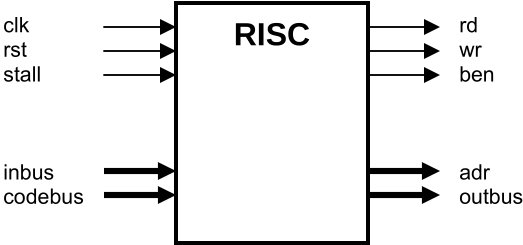
\includegraphics[width=.96\textwidth]{i/F/1.png}
	\caption{The processor's interface}
	\label{fig:processor}
\end{figure}

The main parts of the hardware interface are three busses, the data input and output busses, the
code bus, and the address bus. Signals $rd$ and $wr$ indicate, whether a read or a write operation is to
be performed. $ben$ indicates a byte (rather than word) access. The entire processor operates
synchronously on the clock $clk$ (25 MHz on Spartan-3), $rst$ is the reset signal (from a push button on
the development board), and $stall$ is the input to stall the processor.

First we concentrate on the implementation of the processor core, its realization in the form of
circuits. They are divided into two parts, the Arithmetic/Logic Unit(ALU) processing data, and the control
unit determining the flow of instructions.

\section{The arithmetic and logic unit}
The ALU features a bank of 16 registers with 32 bit words. Arithmetic and logical operations,
represented by instructions, always operate on these registers. Data can be transferred between
memory and registers by separate load and store instructions. This is an important characteristic of
RISC architectures, developed between 1975 and 1985. It contrasts with the earlier CISC
architectures (Complex Instruction Set): Memory is largely decoupled from the processor. A second
important characteristic is that most instructions take a single clock cycle (25 MHz) for their
execution. The exceptions are access to memory, multiplication and division. More about this will be
presented later. This single-cycle rule makes such processors predictable in performance. The
number of cycles and the time required for executing any instruction sequence is precisely defined.
Predictability is essential in all real-time applications.

\begin{figure}[h!]
	\centering
	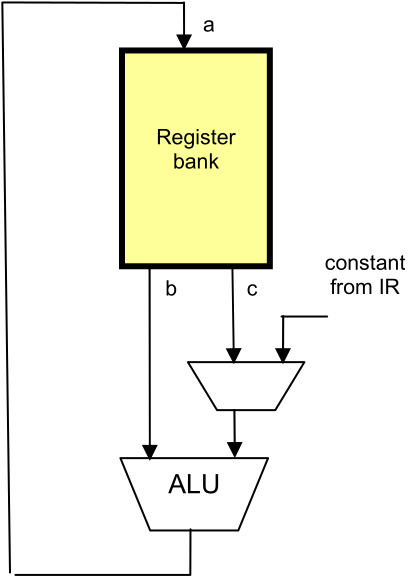
\includegraphics[width=.5\textwidth]{i/F/2.png}
	\caption{Processor core with ALU and registers}
	\label{fig:alu}
\end{figure}

The data processing unit consisting of ALU and registers is shown in Fig \ref{fig:alu}. Evidently, data
cycle from registers through the ALU, where an operation is performed, and the result is deposited
back into a register. The ALU embodies the circuits for arithmetic operations, logical operations,
and shifts. The operations available are listed below. They are described in more detail in
Appendix A2. The operand $n$ is either a register or a part of the instruction itself.

\begin{verbatim}
   0 MOV a,n   R.a:=n
   1 LSL a,b,n R.a:=R.b  ←  n (shift L by n bits)
   2 ASR a,b,n R.a:=R.b  →  n (shift R by n bits
                              with sign extension)
   3 ROR a,b,n R.a:=R.b rot n (rotate R by n bits)

   4 AND a,b,n R.a:=R.b  &  n (logical
   5 ANN a,b,n R.a:=R.b  & ~n  operations)
   6 IOR a,b,n R.a:=R.b  or n (inclusive or)
   7 XOR a,b,n R.a:=R.b xor n (exclusive or)

   8 ADD a,b,n R.a:=R.b  +  n (
   9 SUB a,b,n R.a:=R.b  –  n  integer
  10 MUL a,b,n R.a:=R.b  x  n  arithmetic
  11 DIV a,b,n R.a:=R.b div n )

  12 FAD a,b,c R.a:=R.b + R.c (
  13 FSB a,b,c R.a:=R.b – R.c  floating-point
  14 FML a,b,c R.a:=R.b x R.c  arithmetic
  15 FDV a,b,c R.a:=R.b / R.c )
\end{verbatim}

The following excerpt describes the essence of the ALU circuits. It is written in the HDL Verilog
and refers to the following wires and registers.

\begin{verbatim}
  wire [31:0] IR;  // instruction field(s):
  wire p, q, u, v, w;
      // IR[31], IR[30], IR[29], IR[28], IR[16]
  wire [3:0] op, ira, irb, irc;
      // IR[19:16], IR[27:24], IR[23:20], IR[3:0]
  wire [15:0] imm; // IR[15:0]

  wire [31:0] A, B, C0, C1, regmux;
  wire [31:0] s3, t3, quotient, fsum, fprod, fquot;
  wire [32:0] aluRes;
  wire [63:0] product;

  reg [31:0] R [0:15]; // array of 16 registers
  reg N, Z, C, OV;     // condition flags
\end{verbatim}

$B$ and $C0$ are the outputs from the register bank, and $A$ is its input. The register numbers $ira$ for port
$A$, $irb$ for port $B$, and $irc$ for port $C0$ are taken from 4-bit fields of the instruction register IR. $C1$ is the
multiplexer selecting among the register output $C0$ and the immediate field $imm$. $s3$ and $t3$ are
outputs of the shift units (Sect. 16.2.1). $product$ is the output of the multiplier (16.2.2), $quotient$ and
remainder those of the divider (16.2.3), $fsum$ that of the floating-point adder (16.2.4), $fprod$ that of the
floating-point multiplier (16.2.5), and $fquot$ the output of the floating-point divider (16.2.6).

\begin{verbatim}
  assign A  = R[ira];
  assign B  = R[irb];
  assign C0 = R[irc];
  assign C1 = q ? {{16{v}}, imm} : C0;
\end{verbatim}

The following represents the main instruction decoding and selection of results. The opcodes refer to
specific values of fields p and op of IR. Note that if $x$ then $y$ else $z$ is denoted in Verilog by $x ? y : z$.

\begin{verbatim}
  assign aluRes = MOV
    ? (q ? (~u ? {{16{v}}, imm}
               : {imm, 16'b0})
         : (~u ? C0
               : (~irc[0] ? H
                          : {N, Z, C, OV, 20'b0,
                             8'b01010000})))
    :  LSL  ? t3       // L-shift unit output
    : (ASR
      |ROR) ? s3       // R-shift unit output
    :  AND  ? B & C1
    :  ANN  ? B & ~C1
    :  IOR  ? B | C1
    :  XOR  ? B ^ C1
    :  ADD  ? B + C1 + (u & C)
    :  SUB  ? B - C1 - (u & C)
    :  MUL  ? product [31:0] // multiplier output
    :  DIV  ? quotient
    : (FAD
      |FSB) ? fsum
    :  FML  ? fprod
    :  FDV  ? fquot : 0;
\end{verbatim}

The input to the register bank, $regmux$, is selected from either $aluRes$, inbus (for LDR instructions),
or the program address $nxpc$ (for branch and link instructions). The signal $regwr$ determines,
whether data are to be stored (written) into the register bank. Details must be gathered from the
respective program listing RISC.v.

\begin{verbatim}
  always @ (posedge clk) begin
    R[ira] <= regwr     ?  regmux     : A ;
    N      <= regwr     ?  regmux[31] : N ;
    Z      <= regwr     ? (regmux==0) : Z ;
    C      <= (ADD|SUB) ?  aluRes[32] : C ;
    OV     <= (ADD|SUB) ?  aluRes[32]
                         ^ aluRes[31] : OV;
  end
\end{verbatim}

Whenever a register is written, the condition flags are also affected. They are $N$ ($aluRes$ negative),
$Z$ ($aluRes$ zero), $C$ (carry), and $OV$ (overflow). The latter apply only to addition and subtraction.

\subsection{Shifters}
Shifters are multi-way multiplexers. For a 32-bit word, the simplest solution would be 32 32-way
multiplexers. But this is hardly economical. On the FPGA used here, 4-way muxes are basic cells.
It is therefore beneficial, to compose a shifter out of 4-way muxes. Now the obvious solution is to
use 3 levels of muxes through which data flow. The first level shifts by amounts of 0, 1, 2, or 3, the
second by amounts of 0, 4, 8, 12, and the third by 0 or 16. This scheme is programmed as follows
for left shifts (instruction LSL) with $B$ as input, $sc0 = C1[1:0]$ and $sc1 = C1[3:2]$ as shift counts, and
$t3$ as output:

\begin{verbatim}
  assign t1 = (sc0 == 3) ? { B[28:0],  3'b0} :
              (sc0 == 2) ? { B[29:0],  2'b0} :
              (sc0 == 1) ? { B[30:0],  1'b0} : B ;
  assign t2 = (sc1 == 3) ? {t1[19:0], 12'b0} :
              (sc1 == 2) ? {t1[23:0],  8'b0} :
              (sc1 == 1) ? {t1[27:0],  4'b0} : t1;
  assign t3 =   C1[4]    ? {t2[15:0], 16'b0} : t2;
\end{verbatim}

The solution for right shifts is analogous. An additional level of multiplexing is required, shifting in
either the sign bit (ASR with sign propagation) or bits from the low end of the word (ROR), making
a barrel shifter. This selection is controlled by the instruction bit $w = IR[16]$.

\subsection{Multiplication}
Multiplication is an inherently more complex operation than addition and subtraction. After all,
multiplication can be composed (of a sequence) of additions. There are many methods to
implement multiplication, all – of course – based on the same concept of a series of additions.
They show the fundamental problem of trade-off between time and space (circuitry). Some
solutions operate with a minimum of circuitry, namely a single adder used for all 32 additions
executed sequentially (in time). They obviously sacrifice speed. The other extreme is multiplication
in a single cycle, using 32 adders in series (in space). This solution is fast, but the amount of
required circuitry is high.

Before we present the sequential solution, let us briefly recapitulate the basics of a multiplication $p
:= x × y$. Here $p$ is the product, $x$ the multiplier, and $y$ the multiplicand. Let $x$ and $y$ be unsigned
integers. Consider $x$ in binary form.

\[  x = x_{31}×2^{31} + x_{30}×2^{30} + … + x_1×2^1 + x_0×2^0 \]

Evidently, the product is the sum of 32 terms of the form $x_k×2^k×y$, i.e. of $y$ left shifted by $k$ positions
multiplied by $x_k$. Since $x_k$ is either $0$ or $1$, the product is either $0$ or $y$ (shifted). Multiplication is thus
performed by an adder and a selector. The selector is controlled by $x_k$, a bit of the multiplier.
Instead of selecting this bit among $x_0$ … $x_{31}$, we right shift $x$ by one bit in each step. Then the
selection is always according to $x_0$. The add-shift step then is 
\begin{verbatim}
  IF ODD(x) THEN p := p + y END;
  y := 2*y; x := x DIV 2
\end{verbatim}

whereby multiplication by 2 is done by a left shift, and division by 2 by a right shift: As an example,
consider the multiplication of two 4-bit integers $x = 5$ and $y = 3$, requiring 4 steps:
\begin{table}[h!]
  \centering
  \begin{tabular}{l l l l l}
               & p         & x    & y         \\\hline
               & 0000'0000 & 0101 & 0000'0011 \\
    add y to p & 0000'0011 & 0101 & 0000'0011 \\
    shift      & 0000'0011 & 0010 & 0000'0110 \\
    add 0 to p & 0000'0011 & 0010 & 0000'0110 \\
    shift      & 0000'0011 & 0001 & 0000'1100 \\
    add y to p & 0000'1111 & 0001 & 0000'1100 \\
    shift      & 0000'1111 & 0000 & 0001'1000 \\
    add 0 to p & 0000'1111 & 0000 & 0001'1000 \\
    shift      & 0000'1111 & 0000 & 0011'0000 & p = 15
  \end{tabular}
\end{table}

The shifting of $x$ to the right also suggests that instead of shifting $y$ to the left in each step, we
keep $y$ in the same position and shift the partial sum $p$ to the right. We notice that the size of $x$
decreases by 1 in each step, whereas the size of $p$ increases by 1. This allows to pack $p$ and $x$
into a single double register <$B$, $A$> with a shifting border line. At the end, it contains the product $p
= x × y$.

\begin{table}[h!]
  \centering
  \begin{tabular}{l l r l}
               & p        &    x \\\hline
               & 0000     & 0101 \\
    add y to p & 0011     & 0101 \\
    shift      & 00011    &  010 \\
    add 0 to p & 00011    &  010 \\
    shift      & 000011   &   01 \\
    add y to p & 001111   &   01 \\
    shift      & 0001111  &    0 \\
    add 0 to p & 0001111  &    0 \\
    shift      & 00001111 &      & p = 15
  \end{tabular}
\end{table}
\begin{verbatim}
  p = {B[31:0], A{31:[32-k]},
  x = A[31-k:0]               k = 0 … 31
\end{verbatim}

The multiplier is controlled by a rudimentary state machine $S$, actually a simple 5-bit counter
running from 0 to 31. The multiplier is shown schematically in Fig \ref{fig:multiplier}.

\begin{figure}[h!]
	\centering
	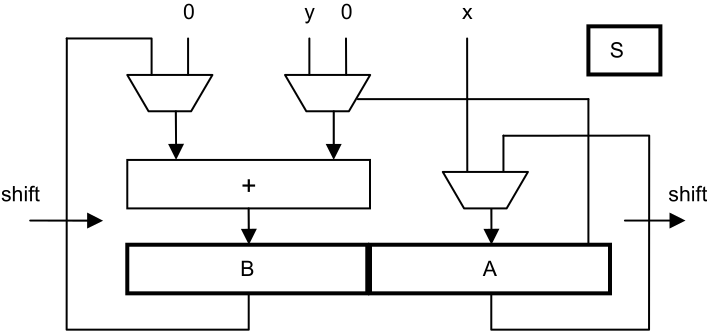
\includegraphics[width=.9\textwidth]{i/F/3.png}
	\caption{Schematic of multiplier}
	\label{fig:multiplier}
\end{figure}

The multiplier interprets its operands as signed ($u = 0$) or unsigned ($u = 1$) integers. The difference
between unsigned and signed representation is that in the former case the first term has a
negative weight ($-x_{31}×2^{31}$). Therefore, implementation of signed multiplication requires very little
change: Term 31 is subtracted instead of added (see complete program listing below).

\begin{verbatim}
  stall = MUL & ~(S == 31);
  S <= MUL ? S+1 : 0;
\end{verbatim}

During execution of the 32 add-shift steps the processor must be stalled. The process proceeds
and the counter $S$ advances as long as the input MUL is active (high). MUL indicates that the
current operation is a multiplication, and the signal is stable until the processor advances to the
next instruction. This happens when step 31 is reached (Fig \ref{fig:stall}).

\begin{figure}[h!]
	\centering
	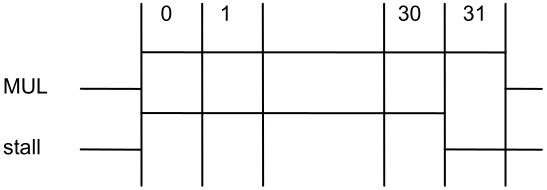
\includegraphics[width=.9\textwidth]{i/F/4.png}
	\caption{Generating $stall$}
	\label{fig:stall}
\end{figure}

The details of the simple multiplier are listed below:

\begin{verbatim}
  module Multiplier(
    input CLK, MUL, u,
    output stall,
    input [31:0] x, y,
    output [63:0] z);
 
  reg [4:0] S; // state
  reg [31:0] B2, A2; // high and low parts of partial product
  wire [32:0] B0, B00, B01;
  wire [31:0] B1, A0, A1;
 
  assign stall = MUL & ~(S == 31);
  assign B00 = (S == 0) ? 0 : {B2[31] & u, B2};
  assign B01 = A0[0] ? {y[31] & u, y} : 0;
  assign B0 = ((S == 31) & u) ? B00 - B01 : B00 + B01;
  assign B1 = B0[32:1];
  assign A0 = (S == 0) ? x : A2;
  assign A1 = {B0[0], A0[31:1]};
  assign z = {B1, A1};
 
  always @ (posedge(CLK)) begin
    B2 <= B1; A2 <= A1;
    S <= MUL ? S+1 : 0;
  end
  endmodule
\end{verbatim}

Implementing multiplication in hardware made the operation about 30 times faster than its solution
by software. A significant factor! As multiplication is a relatively rare operation – at least in
comparison with addition and subtraction – early RISC designs (MIPS, SPARC, ARM) refrained
from its full implementation in hardware. Instead, an instruction called multiply step was provided,
performing a single add-shift step in one clock cycle. A multiplication was then programmed by a
sequence of 32 step instructions, typically provided as a subroutine. This measure of economy
was abandoned, when hardware became faster and cheaper.

The FPGA used on the Spartan-3 board features a welcome facility for speeding up multiplication,
namely fast 18 x 18 bit multiplier units. These are made available as basic cells of the FPGA, and
they multiply in a single clock cycle. Considering an operand $x = x_1×2^{16} + x_0$, the product is
obtained as the sum of only 4 terms:

\[ p = x × y = x_1×y_1×2^{32} + (x_0×y_1 + x_1×y_0)×2^{16} + x_0×y_0 \]

Thereby multiplication of two 32-bit integers can be performed in 2 cycles only, one for
multiplications, one for addition. Four multipliers are needed. For details, the reader is referred to
the program listing (module Multiplier1).

\subsection{Division}
Division is similar to multiplication in structure, but slightly more complicated. We present its
implementation by a sequence of 32 shift-subtract steps, the complement of add-shift. We here
discuss division of unsigned integers only.

\begin{verbatim}
  q = x DIV y
  r = x MOD y
\end{verbatim}

$q$ is the quotient, $r$ the remainder. These are defined by the invariants

\[ x = q×y + r\text{ with }0 \le r < y \]

Both $q$ and $r$ are held in registers. Initially we set $r$ to $x$, the dividend, and then subtract multiples
of $y$ (the divisor) from it, each time checking that the result is not negative. This shift-subtract step is

\begin{verbatim}
  r := 2*r; q := 2*q;
  IF r – y >= 0 THEN r := r – y END
\end{verbatim}

As an example, consider the division of the 8-bit integer $x = 14$ by the 4-bit integer $y = 4$, where
multiplication and division by 2 are done by shifts:

\begin{table}[h!]
  \centering
  \begin{tabular}{l l l l l}
                 & r         & q    & y         \\\hline
                 & 0000'1110 & 0000 & 0001'1000 \\
    shift        & 0000'1110 & 0000 & 0001'1000 & r < y \\
    sub 0 from r & 0000'1110 & 0000 & 0000'1100 \\ 
    shift        & 0000'1110 & 0000 & 0000'1100 & r >= y \\
    sub y from r & 0000'0010 & 0001 & 0000'1100 \\ 
    shift        & 0000'0010 & 0010 & 0000'0110 & r < y \\
    sub 0 from r & 0000'0010 & 0010 & 0000'0110 \\ 
    shift        & 0000'0010 & 0100 & 0000'0011 & r < y \\
    sub y from r & 0000'0010 & 0100 & 0000'0011 & q = 4, r = 2
  \end{tabular}
\end{table}

As with multiplication this arrangement may be simplified by putting r and q into a double-length
shift register, and by shifting r to the left instead of y to the right. This results in

\begin{table}[h!]
  \centering
  \begin{tabular}{l l r l}
                 & r         &    q \\\hline
                 & 0000'1110 &      \\
    shift        & 0001'110  &    0 & r < Y \\
    sub 0 from r & 0001'110  &    0 \\
    shift        & 0011'10   &   00 & r >= Y \\
    sub y from r & 0000'10   &   01 \\
    shift        & 0001'0    &  010 & r < Y \\
    sub 0 from r & 0001'0    &  010 \\
    shift        & 0010      & 0100 & r < Y \\
    sub 0 from r & 0010      & 0100 & q = 4, r = 2
  \end{tabular}
\end{table}

This scheme is represented by the circuit shown in Fig \ref{fig:divider}.

\begin{figure}[h!]
	\centering
	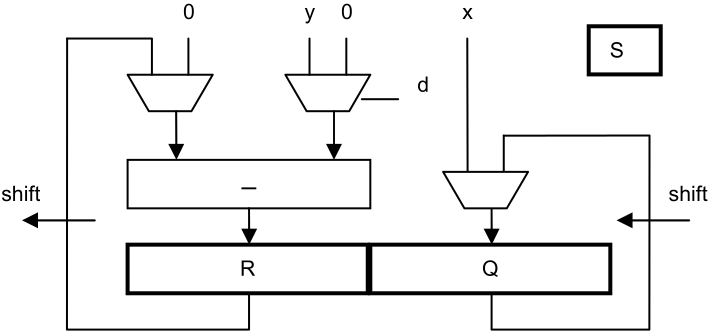
\includegraphics[width=.9\textwidth]{i/F/5.png}
	\caption{Schematic of divider}
	\label{fig:divider}
\end{figure}

Stall generation is the same as for the multiplier. A division takes 32 clock cycles. Further details
are shown in the subsequent program listing.

\begin{verbatim}
  module Divider(
    input clk, DIV,
    output stall,
    input [31:0] x, y,
    output [31:0] quot, rem);
 
  reg [4:0] S; // state
  reg [31:0] r3, q2;
  wire [31:0] r0, r1, r2, q0, q1, d;
 
  assign stall = DIV & ~(S == 31);
  assign r0 = (S == 0) ? 0 : r3;
  assign d = r1 - y;
  assign r1 = {r0[30:0], q0[31]};
  assign r2 = d[31] ? r1 : d;
  assign q0 = (S == 0) ? x : q2;
  assign q1 = {q0[30:0], ~d[31]};
  assign rem = r2;
  assign quot = q1;
  
  always @ (posedge(clk)) begin
    r3 <= r2; q2 <= q1;
    S <= DIV ? S+1 : 0;
  end
  endmodule
\end{verbatim}

\section{Floating-point arithmetic}
The RISC uses the IEEE Standard for representing REAL (floating-point) numbers with 32 bits.
The word is divided into 3 fields: s for the sign, e for the exponent, and m for the mantissa. The
value is 

\[ x = (-1)^s × 2^{-127} × 1.m\text{ with }1.0 \le m < 2.0\text{ (normalized form)} \]

Numbers are represented in sign-magnitude form. This implies that for sign inversion only the sign
bit must be inverted, and exponent and mantissa remain unchanged.

Zero is a special case represented by 32 0-bits, and therefore has to be treated separately.
Furthermore, e = 255 denotes "not a number". It is generated in the case of arithmetic overflow.

\begin{figure}[h!]
	\centering
	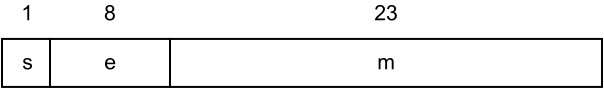
\includegraphics[width=.9\textwidth]{i/F/6.png}
	\caption{IEEE standard floating-point representation of REAL numbers}
	\label{fig:float-point}
\end{figure}

\subsection{Floating-point addition}
If two numbers are to be added, they must have the same exponent. This implies that the
summand with the smaller exponent must be denormalized. m is shifted to the right and e is
incremented accordingly. That is, if d is the difference of the two exponents, m is multiplied by 2d,
and e is incremented by d. After the addition, the sum must be rounded and post-normalized. m is
shifted to the left and e is decremented accordingly. The shift amount is determined by the
position of the leftmost one-bit. This results in the scheme shown in Fig 16.7, and the module's
interface is

\begin{verbatim}
  module FPAdder(
    input clk, run, u, v,
    input [31:0] x, y,
    output stall,
    output [31:0] z);
\end{verbatim}
\begin{figure}[h!]
	\centering
	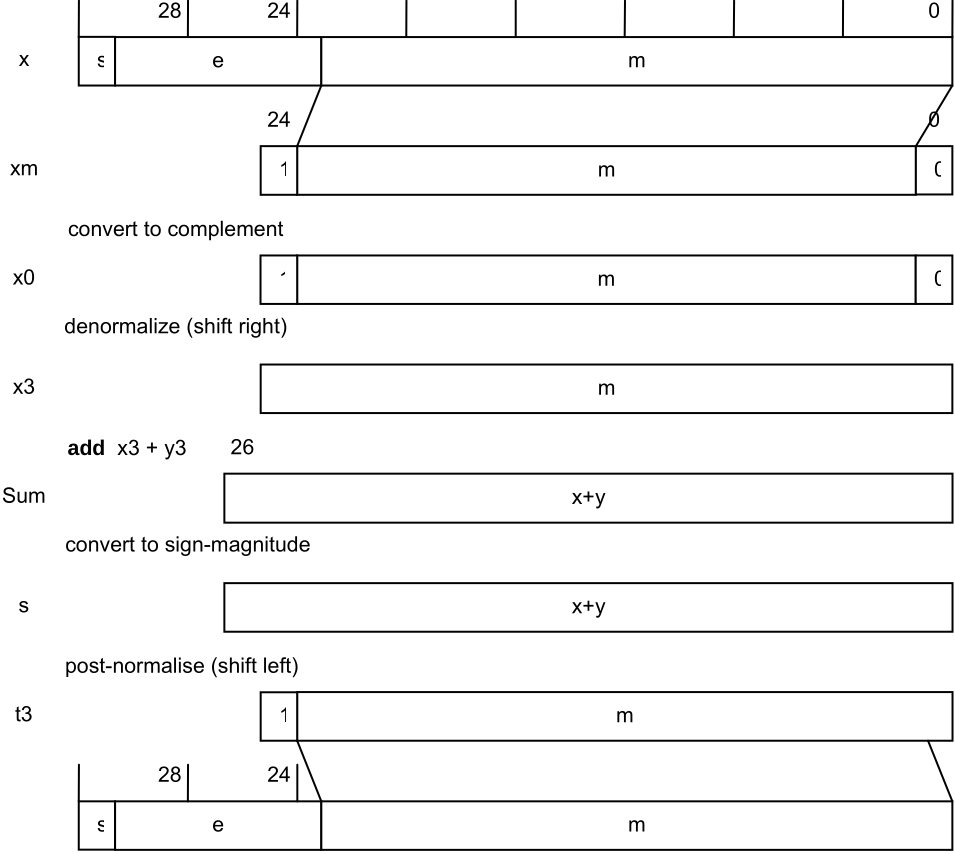
\includegraphics[width=.9\textwidth]{i/F/7.png}
	\caption{Steps of floating-point addition}
	\label{fig:fpaddition}
\end{figure}

It is important to achieve proper rounding. This is done by extending the mantissa of both
operands by a guard bit, initialized to 0. A one is added (effectively 0.5) and at the end the guard
bit is discarded.

The two predefined conversion functions FLT and FLOOR are conveniently implemented as
additions. A denormalized 0 is added to the argument, effecting the proper shift. In the case of
FLT (modifier bit u = 1), denormalization is omitted (no 1-bit inserted), and in the case of FLOOR
(modifier bit v = 1), post-normalization is suppressed.

\subsection{Floating-point multiplication}
A product is given by the equation

\[ p = x × y = (2^{xe} × xm) × (2^{ye} × ym) = 2^{xe+ye} × (xm * ym) \]
\[ p = (xs, xe, xm) × (ys, ye, ym) = (xs\text{ xor }ys, xe + ye, xm × ym) \]

That is, exponents are added, mantissas multiplied. Denormalization is not needed. Post-
normalization is a right shift of at most one bit, because if 1.0 $\le$ xm, ym < 2.0, the result satisfies
1.0 $\le$ xm*ym < 4.0. The sign of the product is the exclusive or of the signs of the arguments. The
multiplier module's interface is

\begin{verbatim}
  module FPMultiplier(
    input clk, run,
    input [31:0] x, y,
    output stall,
    output [31:0] z);
\end{verbatim}

\subsection{Floating-point division}
A quotient is given by the equation

\begin{verbatim}
  module FPDivider(
    input clk, run,
    input [31:0] x, y,
    output stall,
    output [31:0] z);
\end{verbatim}

\section{The Control Unit}
\[ q = x / y = (2^{xe} × xm) / (2^{ye} × ym) = 2^{xe-ye} × (xm / ym) \]
\[ q = (sx, ex, mx) / (sy, ey, my) = (sx\text{ xor }sy, ex - ey, mx / my) \]

That is, exponents are subtracted, mantissas divided. Denormalization is not needed. Post-
normalization requires a left shift by at most a single bit, because if $1.0 \le xm, ym < 2.0$, the result
satisfies $0.5 \le xm/ym < 2.0$. The sign of the product is the exclusive or of the signs of the
arguments. The divider module's interfaces is

The control unit determines the sequence of executed instructions. It contains two registers, the
program counter PC holding the address of the current instruction, and the current instruction
register IR holding the instruction currently being interpreted. Instructions are obtained from
memory through the codebus (see interface), from where the decoding signals emanate. Mostly,
the arithmetic unit and the control unit operate concurrently (in parallel). While the arithmetic unit
performs the operation held in register IR and data signals flow through the ALU, the control unit
fetches in the same clock cycle the next instruction from memory in the location with the address
held in PC. Next address and next instruction are latched in the registers at the end of a cycle.
This scheme constitutes a one-element pipeline of instructions.

The principal task of the control unit is to generate the address of the next instruction. There are
essentially only four cases:

\begin{enumerate}
  \item Zero on reset.
  \item The next instructions address is PC+1 (all instructions except branches)
  \item The branch target PC+1 + offset. (Branch instructions).
  \item It is taken from a data register. (This is used for returning from procedures).
\end{enumerate}

This is reflected by the following program text, and shown in Fig \ref{fig:cu}.

\begin{figure}[h!]
	\centering
	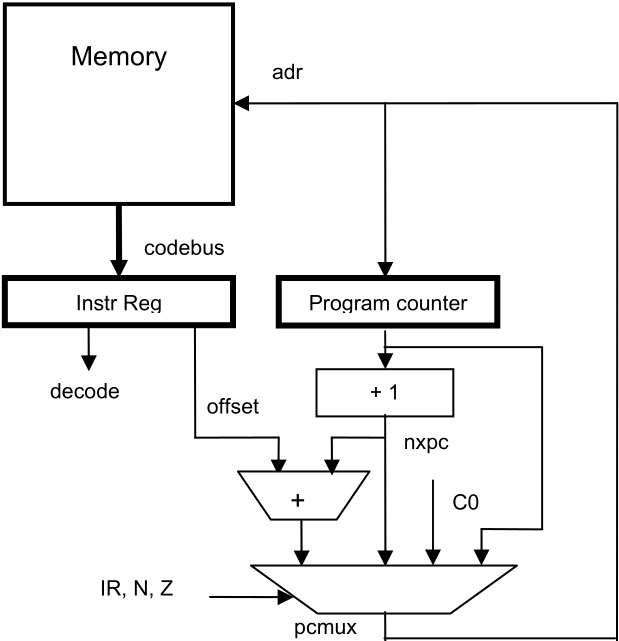
\includegraphics[width=.9\textwidth]{i/F/8.png}
	\caption{The control unit}
	\label{fig:cu}
\end{figure}

\begin{verbatim}
  reg [17:0] PC;
  reg [31:0] IRBuf;
  wire [31:0] IR;
  wire [31:0] pmout;
  wire [17:0] pcmux, nxpc;
  wire cond;
 
  IR = codebus;
  nxpc = PC + 1;
  pcmux = (~rst) ? 0 :
      (stall) ? PC : // stall
      (BR & cond & u) ? off + nxpc :
      (BR & cond & ~u) ? C0[19:2] :
      nxpc;
 
  always @ (posedge clk) PC <= pcmux; end
\end{verbatim}

Branches are the only conditional instructions. Whether a branch is taken or not, is determined by
the combination of the condition flags selected by the condition code field of the branch
instruction. IR[27] is the condition sense inversion bit.

\begin{verbatim}
  reg N, Z, C, OV; // condition flags
  wire S;
  assign S = N ^ OV;
  assign cond = IR[27] ^
      ((cc == 0) &   N   |  // MI, PL
       (cc == 1) &   Z   |  // EQ, NE
       (cc == 2) &   C   |  // CS, CC
       (cc == 3) &  OV   |  // VS, VC
       (cc == 4) & (C|Z) |  // LS, HI
       (cc == 5) &   S   |  // LT, GE
       (cc == 6) & (S|Z) |  // LE, GT
       (cc == 7));          //  T, F
\end{verbatim}

There is, unfortunately, a complication obfuscating the simple scheme presented so far. It stems
from the necessity to initialize the processor. Only registers and memory blocks (BRAM) can be
initialized and loaded by the available FPGA-tools. How, then, is a program (in our case the boot
loader) moved into memory, the chip-external SRAM? The following scheme has been chosen:

The initial program is loaded into a BRAM (1K x 32). This block is memory-mapped into high-end
addresses in the range of the data stack. On startup, the flag PMsel is set and IR is loaded from
pmout (from the BRAM) at StartAdr. At the end of the program (boot loader), a branch instruction
with destination 0 jumps to the beginning of the program that had just been loaded into SRAM by
the boot loader. This is, presumably, but not necessarily, the operating system. The following
changes and additions are required:

\begin{verbatim}
  localparam StartAdr = 18'b111111100000000000; // 0FE000H

  reg PMsel; // memory select for instruction fetch
  reg [31:0] IRBuf;

  dbram32 PM ( // BRAM
      .clka (clk),
      .rdb (pmout), // output port
      .ab (pcmux[10:0])); // address

  assign IR = PMsel ? pmout : IRBuf;

  always @ (posedge clk) begin
    PMsel <= ~rst | (pcmux[17:11] == 7'b1111111);
    IRBuf <= stall ? IRBuf : codebus;
    ...
  end;
\end{verbatim}
